\section{Tests}

The tests made for this project is primarily done with unit
tests. The program user interface has been tested by hand.

\subsection{Unit Test 1 - Add new class}

The user may want to add a new class to the model. By pressing the button, it is
possible to observe that a new class indeed appears. The test tests to see if a
new \texttt{Klass} instance has been added to the \texttt{MainViewModel}'s
collection.

\subsection{Unit Test 2 - Remove class}

The user may also want to remove a class from the diagram. In this case, it is
necessary to first select a class, and then call remove.

It is then asserted that the class is removed from the \texttt{Klasses}
collection.

It is also tested for the case when no class is selected. In this case, nothing
should happen.

Instead of letting nothing happen, it would be possible to throw an exception.
This would also make it possible to warn the user if necessary.

\subsection{Unit Test 3 - Copy/Paste class}

This test is to make sure that the copy pasted class is added to the viewmodel,
and that it is a deep copy.

This functionality also relies on a selected class, so it is also tested that
nothing happens when no class is selected.

The user may also want to paste a class multiple times. These extra copies does
also have to be deep copies, and the user should be able to paste multiple times
without having to reselect a class.


\subsection{Unit Test 4 - Setting a relation}

The user should be able to add a relation between 2 models. It is crucial for
the model, that a relation has a reference to each class, and that each class has
a reference to each relation.

The test makes sure that it happens.

\subsection{Unit Test 5 - Unsetting a relation}

It is possible to remove a relation. Since this affects the state of the program
multiple places when set, they all have to be reverted when unset.


\subsection{Code coverage}

\begin{figure}
\centering
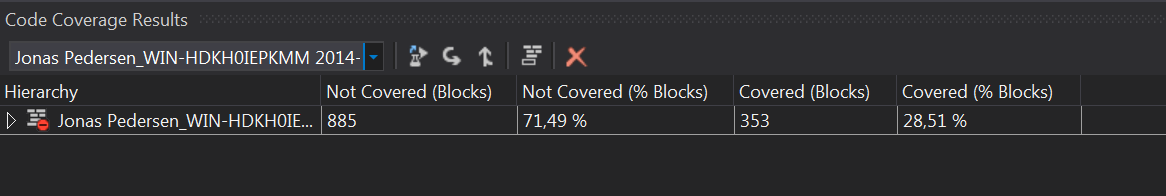
\includegraphics[width=0.85\linewidth]{img/coverage}
\caption{Screenshot of the Visual Studio code coverage tools result.}
\end{figure}

The tests cover approximately $30\%$ of all the code. Achieving $100\%$ would
likely take as long time as making the project itself, so only the most
important, and most likely to break stuff, was tested.

It would also be difficult to test the GUI part of the program, and since e.g.
AddRelation relies on mouse clicks, it would be hard to make unit test for.
